\section{Windows GUI}
Implementeringen af den grafiske bruger grænseflade til Windows PC applications program beskrives her.
Kildekoden ligger i projektet Application.Win.
\subsection{WinLoginView}
Første skærm eller view der vises er WinLoginView.
\begin{figure}
	\centering
	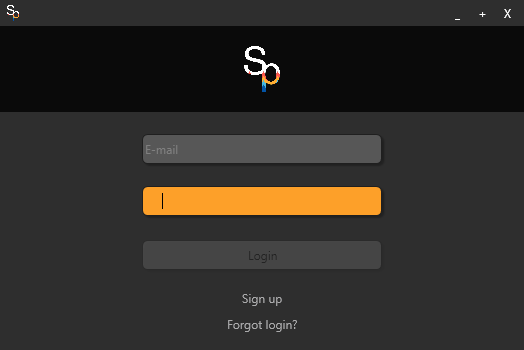
\includegraphics[width=0.7\linewidth]{figs/implementering/winloginview}
	\caption{WinLoginView}
	\label{fig:winloginview}
\end{figure}
Det var blevet besluttet at textbox'ene skulle have "placeholder" text, hvilket ikke findes som standard i WPF. Placeholder tekst fortæller hvad det er forventet brugeren skriver i feltet. På figur~\ref{fig:winloginview} ses det i øverste felt at brugeren skal skrive sin e-mail. Placeholder teksten forsvinder, når brugeren skriver i feltet, hvilket ses i felt nummer to til password. Password teksten er hemmelig og derfor ikke synlig. 

Det blev overvejet om det var forsvarligt at have passwordet i en normal textbox, i stedet for en WPF PasswordBox, hvor indholdet ikke ligger ukrypteret i hukommelsen. 
For at sende passwordet til severen, skal det alligevel være ukrypteret, så det ville ikke ændre meget på sikerheden. Derfor blev diskussionen droppet.

Placeholder teksten er lavetog vist ved hjælp af en property og en template til en normal TextBox.
Placeholder teksten er lavet som en property, som kan sættes på alle controls med klassen ThemeProperties der ligger i WinLoginView.xaml.cs. Det ses i følgende kode udsnit.
\begin{lstlisting}[caption=ThemeProperties, label=code:ThemeProperties]
public static class ThemeProperties
{
public static string GetPlaceholderText(DependencyObject obj)
{
return (string)obj.GetValue(PlaceholderTextProperty);
}

public static void SetPlaceholderText(DependencyObject obj, string value)
{
obj.SetValue(PlaceholderTextProperty, value);
}

public static readonly DependencyProperty PlaceholderTextProperty =
DependencyProperty.RegisterAttached(
"PlaceholderText",
typeof(string),
typeof(ThemeProperties),
new FrameworkPropertyMetadata("Placeholder"));
}
\end{lstlisting} 
Med SetPlaceholderText() kan man så sætte placeholder teksten til en given control.
Det kunne have været lavet som en PlaceholderTextBox klasse ligesom StatViewer i figur~\ref{code:StatViewer}, men dette blev lavet inden den idé opstod.

Placeholder teksten bliver vist, fordi den er en templateBinding til den i en template til TextBox'ene. Implementeringen af templaten ses her.
\begin{lstlisting}[caption=TextBoxWPlaceholderTemplate, label=code:TextBoxWPlaceholderTemplate]
<!-- TextBox with a placeholder containing attached property PlaceholderText-->
<ControlTemplate x:Key="TextBoxWPlaceholderTemplate" TargetType="{x:Type TextBox}">
<Grid>
<Border Background="{StaticResource SpGrey}" x:Name="Bd" BorderBrush="{StaticResource SpDarkGrey}" BorderThickness="{TemplateBinding BorderThickness}" CornerRadius="5" Height="30" >
<ScrollViewer x:Name="PART_ContentHost"/>
<Border.Effect>
<DropShadowEffect Color="Black" Direction="320" ShadowDepth="3" BlurRadius="2" Opacity="0.3" />
</Border.Effect>
</Border>

<TextBlock IsHitTestVisible="False" Text="{Binding Path=(local:ThemeProperties.PlaceholderText), RelativeSource={RelativeSource TemplatedParent}}" 
VerticalAlignment="Center" HorizontalAlignment="Left" Margin="3,0,0,0" Foreground="#FF808080">
<TextBlock.Style>
<Style TargetType="{x:Type TextBlock}">
<Setter Property="Visibility" Value="Collapsed"/>
<Style.Triggers>
<DataTrigger Binding="{Binding RelativeSource={RelativeSource TemplatedParent}, Path=Text}" Value="">
<Setter Property="Visibility" Value="Visible"/>
</DataTrigger>
</Style.Triggers>
</Style>
</TextBlock.Style>
</TextBlock>
</Grid>
...
\end{lstlisting}
På linje 11 er en TextBlock der er båndet til placeholder teksten tilføjet til TextBox'en. 
På linje 17 er der lavet en DataTrigger. Den er båndet til teksten i TextBox'en. Hvis tekst property'en er tom, vises placeholder teksten.
\subsection{WinStatView}
Til at vise nuværende data blev WinStatView lavet.
\begin{figure}[h]
	\centering
	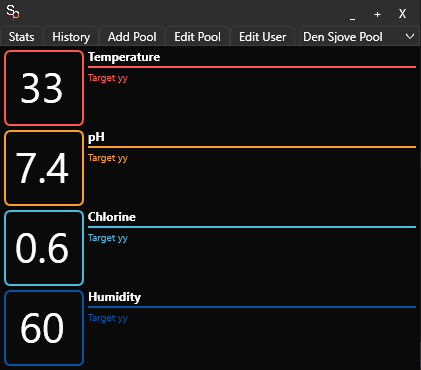
\includegraphics[width=0.5\linewidth]{figs/implementering/winstatview}
	\caption{WinStatView}
	\label{fig:winstatview}
\end{figure}

En controller oprettes, som kan hente de nuværende data. Når ViewDidLoad bliver kaldt på controlleren kalder den følgende funktion.

\begin{lstlisting}[caption=DisplaySensorData(),label=code:DisplaySensorData]
public void DisplaySensorData(List<Tuple<SensorTypes, double>> sensorData)
{
   	foreach (var sensor in sensorData)
   	{
   		switch (sensor.Item1)
   		{
   			case SensorTypes.Temperature:
   			TemperatureStatViewer.Parameter = string.Format($"{sensor.Item2}");
   			break;
   			case SensorTypes.Ph:
   			PhStatViewer.Parameter = string.Format($"{sensor.Item2}");
   			break;
   			case SensorTypes.Chlorine:
   			ChlorineStatViewer.Parameter = string.Format($"{sensor.Item2}");
   			break;
   			case SensorTypes.Humidity:
   			HumidityStatViewer.Parameter = string.Format($"{sensor.Item2}");
   			break;
   		} 
   	}
}
\end{lstlisting}

Den korrekte StatViewer vælges og dens Parameter sættes til at være det nyeste data.

En StatViewer er en custom wpf control, som er lavet til dette formål. Den har en farve der repræsenterer sensor typen, og tekstfelter til property'en Parameter, hvori nuværende data er, Target værdi og sensor typen. 
På figur~\ref{fig:winstatview} ses fire StatViewers. En til hver sensor. 

StatViewer klassen er givet fire ekstra properties. I koden nedenfor ses et eksempel.

\begin{lstlisting}[caption=StatViewer attatched property, label=code:StatViewer]
public class StatViewer : Button
{
	public string Parameter
	{
		get { return (string)GetValue(ParameterProperty); }
		set { SetValue(ParameterProperty, value); }
	}
	
	public static readonly DependencyProperty ParameterProperty =
	DependencyProperty.RegisterAttached(
	"Parameter",
	typeof(string),
	typeof(StatViewer),
	new FrameworkPropertyMetadata("XX"));
	...
\end{lstlisting}

På denne måde er properties til BorderColor, Parameter og ParameterTarget tilføjet til klassen StatViewer. ParameterTarget er der, fordi det var planlagt, at den skulle vise den ønskede værdi, men det er ikke implementeret.

Udseendet på StatViewer er defineret i en template der ligger i StatViewerTheme.xaml. Det er et ResourceDictionary, hvilket tillader at adskille Resourcer fra vinduerne i xaml.
Templaten ses nedenfor.

\begin{lstlisting}[caption=StatViewerTheme, label=code:StatViewerTheme]
<!-- StatView template -->
<Style x:Key="{x:Type local:StatViewer}" TargetType="{x:Type local:StatViewer}">
<Setter Property="Foreground" Value="{StaticResource SpWhite}"/>
</Style>
<ControlTemplate x:Key="StatViewer" TargetType="local:StatViewer">
<Grid Height="80">
<Grid.ColumnDefinitions>
<ColumnDefinition Width="84"/>
<ColumnDefinition Width="*"/>
</Grid.ColumnDefinitions>
<Grid.RowDefinitions>
<RowDefinition Height="18"/>
<RowDefinition Height="6"/>
<RowDefinition Height="*"/>
<RowDefinition Height="22"/>
</Grid.RowDefinitions>
<Border Grid.Row="0" Grid.RowSpan="4" Grid.Column="0" Background="#00000000" Width="80" HorizontalAlignment="Left" BorderThickness="2" BorderBrush="{TemplateBinding BorderColor}" CornerRadius="5" Margin="4, 4, 0, 0"/>
<TextBlock Text="{TemplateBinding Content}" Grid.Row="0"  Grid.Column="1" HorizontalAlignment="Left" Foreground="{TemplateBinding Foreground}"  Margin="4,2,0,0" FontWeight="Bold" />
<Rectangle Grid.Row="1" Grid.Column="1" Height="2" Fill="{TemplateBinding BorderColor}" Margin="4, 0" />
<TextBlock Grid.Row="0" Grid.RowSpan="4" Grid.Column="0" Text="{TemplateBinding Parameter}" Foreground="{TemplateBinding Foreground}" HorizontalAlignment="Center" Margin="0,0,0,0" VerticalAlignment="Center" FontSize="42"/>
<TextBlock Grid.Row="2" Grid.Column="1" Text="{TemplateBinding ParameterTarget}" Foreground="{TemplateBinding BorderColor}" HorizontalAlignment="Left" VerticalAlignment="Top" Margin="4,0,0,0" FontSize="10"/>
</Grid>
</ControlTemplate>
\end{lstlisting}

Bemærk TargetType="local:StatViewer". Templaten er til StatViewer og de steder der står TemplateBinding forbindes de properties der var blevet tilføjet.

\subsection{WinHistoryView}
Til at præsentere brugeren for måledata grafisk i PC applikationen er WinHistoryView lavet.
\begin{figure}
\centering
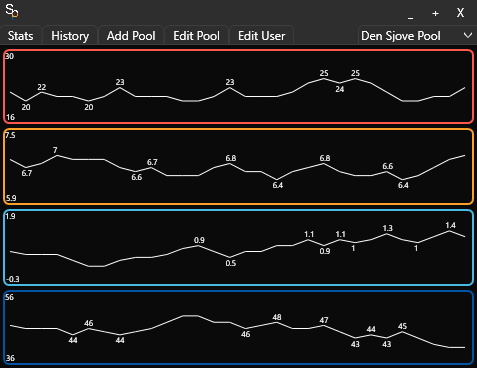
\includegraphics[width=0.6\linewidth]{figs/implementering/winhistoryview}
\caption{WinHistoryView}
\label{fig:winhistoryview}
\end{figure}
Hver graf præsenterer historisk data for en sensor.
Graferne var svære at implementere. De er ikke lavet med specielle controls eller templates, fordi det basale udseende blot er en border med et canvas i. I stedet genererer funktionen DisplayGraph() useendet ud fra modtaget data i runtime. Specielle udsnit af funktionen vises nedenfor.

\begin{lstlisting}[caption=DisplayGraph, label=DisplayGraph]
	private void DisplayGraph(Canvas historyCanvas, List<double> history, bool isPhOrChlorine)
	{
	...
	// Draw graph
	for (var i = 0; i < _pointsOnGraphs; i++)
	{
	Dispatcher.Invoke(() =>
	{
	var pointHeight = ((upperBound - history[i])) / (upperBound - lowerBound) * canvasHeight;
	var pointWidth = (canvasWidth/(_pointsOnGraphs - 1))*i;
	
	...
	
	valueText.Text = history[i].ToString();
	valueText.FontSize = 8;
	historyCanvas.Children.Add(valueText);
	//if valueText belongs to a local minimum it's drawn below the point. Else above
	Canvas.SetTop(valueText, valueTextIsLocalMinimum? pointHeight + 1 : pointHeight - 10);
	Canvas.SetLeft(valueText, pointWidth - 3);
	
	//Draw tendency line
	if (!(i == 0))
	{
	var line = new Line();
	line.StrokeThickness = 1;
	line.Stroke = new SolidColorBrush(Color.FromRgb(0xFF, 0xFF, 0xFF));
	line.X1 = lastPointX;
	line.Y1 = lastPointY;
	line.X2 = pointWidth + 1;
	line.Y2 = pointHeight + 1;
	
	historyCanvas.Children.Add(line);
	Canvas.SetTop(line, lastPointTop + (line.Height/2));
	}
	...
\end{lstlisting}
Funktionen er en hjælpe funktion, der modtager historisk data og tegner en graf på et modtaget canvas.
På linje 9 og 10 udregnes punktets position relativt i forhold til canvas'ets størrelse. 
\_pointsOnGraphs er en variabel der blot er sat til antallet af punkter i det historiske data der er modtaget. Så uanset hvor meget data funktionen modtager, så tegner den det. Der kunne have været implementeret et input felt, hvor brugeren kunne specificere hvor mange dages data han ville se, men det blev ned prioriteret. 
Linje 14 til 19 indsættes punktet i grafen.

\subsection{TabBar}
TabBaren, som ses på alle views efter brugeren har logget ind, er ikke en standard WPF control. WPF har en TabBarControl, men den indeholder pages, som kan indeholde yderligere controls. I views'ne skulle der bruges buttons, som åbnede nye views, når man klikkede. Visuelt giver de indtrykket af at det er en standard tabBar, men funktionaliteten og udseendet er special lavet.
\begin{figure}
\centering
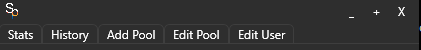
\includegraphics[width=0.7\linewidth]{figs/implementering/tabbar}
\caption{Win tabBar}
\label{fig:tabbar}
\end{figure}
Den er i xaml lavet på samme måde som f.eks. figur~\ref{code:TextBoxWPlaceholderTemplate}, i et ResourceDictionary med en template. 
Templaten indeholder buttons, hvilket voldte problemer. De buttons' click events kunne ikke ses udenfor den overliggende control. Der blev lavet events, som SpTabControl genererer, når buttons'ne bliver clicked.
I SpTabControl.xaml.cs ligger den tilhørende klasse SpTabControl.
\begin{lstlisting}[caption=SpTabControl, label=SpTabControl]
public class SpTabControl : Button
{
	// button objects
	private Button _showStatViewbutton;
	
	// events exposed to container
	public static readonly RoutedEvent OnShowStatButtonClickedEvent =
	EventManager.RegisterRoutedEvent("OnShowStatButtonClicked", RoutingStrategy.Direct, typeof(RoutedEventHandler), typeof(SpTabControl));
	
	static SpTabControl()
	{
		DefaultStyleKeyProperty.OverrideMetadata(typeof(SpTabControl), new FrameworkPropertyMetadata(typeof(SpTabControl)));
	}
	
	// Get the button objects as the template is applied and add click event handlers
	public override void OnApplyTemplate()
	{
		base.OnApplyTemplate();
		
		_showStatViewbutton = GetTemplateChild("PART_StatViewButton") as Button;
		
		if (_showStatViewbutton != null)
			_showStatViewbutton.Click += ShowStatButtonClicked;
	}
	
	// Expose and raise 'OnShowStatButtonClicked' event
	public event RoutedEventHandler OnShowStatButtonClicked
	{
		add { AddHandler(OnShowStatButtonClickedEvent, value); }
	
		remove { RemoveHandler(OnShowStatButtonClickedEvent, value); }
	}
	
	private void ShowStatButtonClicked(object sender, RoutedEventArgs e)
	{
		RaiseEvent(new RoutedEventArgs(OnShowStatButtonClickedEvent));
	}
}
\end{lstlisting}

Koden er skåret ned til kun at vise opsætningen af ét event. Der er et tilsvarende for alle tabs. Se kommentarerne i koden for forklaring.
Der er fundet inspiration på en blog af Alan Beech~\cite{alanbeech2011}.

Når SpTabControl genererer et synligt event kan det fanges af en event handler i codebehind af et vindue. Nedenfor ses det.
\begin{lstlisting}[caption=EventHandler setup, label=EventHandlerSetup]
	//Sets up the tabBars event handlers
	SpTabControl1.OnShowStatButtonClicked += TabBarController.ShowStatButtonPressed;
\end{lstlisting}
Det er placeret i constructoren af alle views med en tabBar.
Funktionen TabBarController.ShowStatButtonPressed() er placeret i klassen TabBarController for at kunne genbruge funktionen i alle views.

\subsection{Vindue design}
Vinduernes udseende er ikke standard .NET. Det er lavet i samme stil som resten af det visuelle design ved hjælp af nogle klasser og en template lavet af Jay Chase~\cite{websiteCustomWindow} på msdn.
Når man fjerner .NETs normale vindue forsvinder den indbyggede funktionalitet også. Det vil sige evnen til at flytte og resize vinduet. I klasserne fra Jay Chase er det lavet, og det er uændret. Klasserne ligger i mappen StyleableWindow. Templaten der beskriver udseendet er stærkt ændret for at få det ønskede udseende.